\documentclass[preprint,12pt]{elsarticle}

\usepackage[utf8]{inputenc}
\usepackage{amsmath,amssymb,amsfonts,amsthm}
\usepackage{booktabs}
\usepackage{multirow}
\usepackage{array}
\usepackage{float}
\usepackage{xcolor}
\usepackage{algorithm}
\usepackage{algorithmic}
\usepackage{tikz}
\usepackage{pgfplots}
\usepackage{subcaption}
\usepackage{hyperref}
\usepackage{cleveref}

\pgfplotsset{compat=1.18}
\journal{Expert Systems with Applications}
\makeatletter
\pdfstringdefDisableCommands{%
  \def\corref#1{}%
  \def\cnotenum#1{}%
  \def\@corref#1{}%
}
\makeatother

\newtheorem{theorem}{Theorem}[section]
\newtheorem{lemma}[theorem]{Lemma}
\newtheorem{proposition}[theorem]{Proposition}
\newtheorem{definition}[theorem]{Definition}
\newtheorem{remark}[theorem]{Remark}

\newif\ifanonymized
\anonymizedtrue
% Set \anonymizedfalse after review to compile the identified version.

\begin{document}

\begin{frontmatter}

\title{A Hybrid Population PDHG Heuristic\\ for Feasibility Recovery in Mixed-Integer Programming}
\ifanonymized
\author{Anonymous Author(s)}
\else
\author[a,b]{Jin Xin Cao\corref{cor1}}
\cortext[cor1]{Corresponding author.}
\ead{imucjx@163.com}
\address[a]{Inner Mongolia Academy of Science and Technology, Hohhot 010010, China}
\address[b]{Institute of Transportation Engineering, Inner Mongolia University, Hohhot 010010, China}
\fi

\begin{graphicalabstract}
\centering
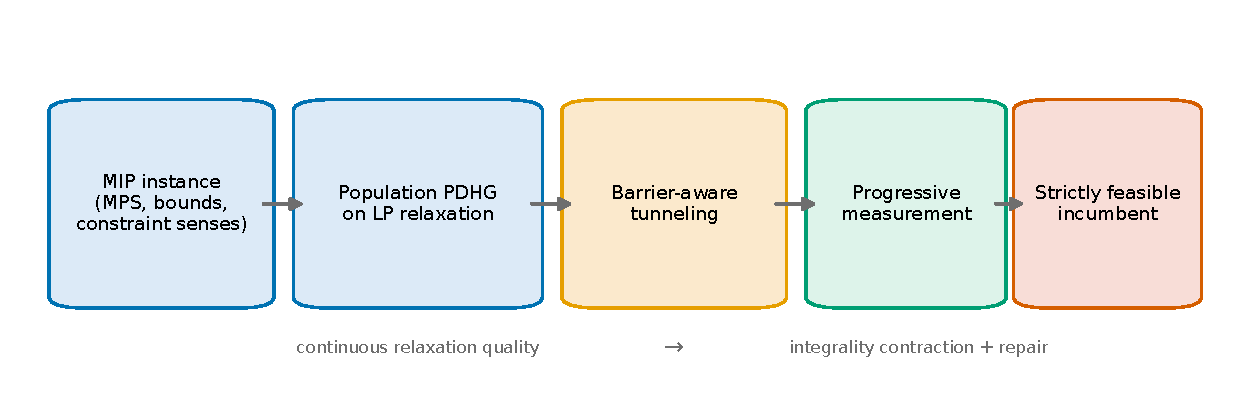
\includegraphics[width=\textwidth]{figures/graphical_abstract_nature.pdf}
\end{graphicalabstract}

\begin{abstract}
Mixed-integer programming (MIP) often becomes difficult in practice not because the relaxation is uninformative, but because fractional trajectories fail to cross the last barrier to feasibility. We propose a hybrid population primal-dual hybrid gradient heuristic (HP-PDHG) that combines population PDHG relaxation search with a barrier-crossing perturbation, progressive projection toward integrality, and feasibility-aware repair. Although one perturbation mechanism is inspired by WKB-style tunneling, the method is classical and serves as a feasibility-recovery heuristic. On the audited four-instance benchmark, HP-PDHG returns feasible incumbents on all four cases, whereas the matched population-PDHG baseline is infeasible on all four. In a 20-seed robustness study (80 paired runs), HP-PDHG achieves 80/80 feasible outcomes versus 0/80 for the baseline, with paired sign-test $p=8.27\times10^{-25}$ and paired Wilcoxon $p=2.75\times10^{-15}$. On a 12-instance official MIPLIB 2017 extension evaluated over five seeds, HP-PDHG reduces mean audited violation on 8 instances, ties on 2, loses on 2, and wins the per-instance Wilcoxon test ($p=0.032$); the largest reductions occur on p200x1188c (81.8\%), neos-3046615-murg (62.7\%), and neos-2657525-crna (53.6\%). On a six-instance subset benchmarked against GA, DE, SHADE, SL-PSO, and a population-PDHG baseline, HP-PDHG attains the best average Friedman rank (1.75), although Holm-adjusted pairwise tests remain conservative. Ablation shows that progressive projection and repair are decisive, while the barrier-crossing perturbation mainly broadens exploration. A 390-run sensitivity study indicates a broad plateau rather than a narrow optimum. These results support HP-PDHG as a MIP feasibility heuristic.
\end{abstract}

\begin{keyword}
Mixed-integer programming \sep primal heuristics \sep first-order methods \sep population search \sep feasibility recovery \sep intelligent optimization
\end{keyword}

\end{frontmatter}

\section{Introduction}
\label{sec:introduction}
Mixed-integer programming (MIP) remains one of the most expressive paradigms for decision optimization because it unifies continuous resource allocation and discrete strategic choice in a single mathematical model \cite{bertsimas2005optimization,morrison2016branch}. This modeling power explains why MIP appears in production planning, scheduling, routing, energy systems, finance, network design, and increasingly in data-driven decision pipelines. The same integrality structure that makes MIP valuable, however, also creates its central computational difficulty. Feasible regions become fragmented, strong linear-relaxation solutions can remain stubbornly fractional, and promising trajectories may fail at the last step from near-feasible to strictly feasible solutions. In many operational settings, that final transition matters more than early claims about ultimate optimality, because a strong feasible incumbent is what enables real decision support and strengthens the downstream exact search.

Modern branch-and-bound and branch-and-cut solvers address this difficulty by combining multiple layers of algorithmic intelligence, including presolve, cutting planes, branching strategies, node selection, and primal heuristics \cite{achterberg2009constraint,gleixner2021miplib}. Among these ingredients, primal heuristics are especially important because they determine whether a promising relaxation can be converted quickly enough into a useful incumbent \cite{berthold2013measuring}. Classical mechanisms such as the feasibility pump, local branching, and relaxation-induced neighborhood search all exploit the same underlying insight: the relaxation already contains structural information that should guide the combinatorial search \cite{fischetti2005feasibility,fischetti2003local,danna2005exploring}. Yet these heuristics also reveal a common limitation. When the feasible mixed-integer region is thin or separated from attractive fractional points by concentrated pockets of violation, local rounding and neighborhood restriction can become brittle, repeatedly revisiting similar infeasible patterns without reliably closing the final feasibility gap.

First-order optimization offers a complementary advantage on the relaxation side of the problem. Primal-dual hybrid gradient (PDHG) methods use sparse matrix-vector operations and simple projections, which makes them attractive on large and sparse relaxations for which repeated factorizations are expensive or memory intensive \cite{chambolle2011first,applegate2021practical,lu2023cupdlp}. Recent large-scale linear-programming systems show that carefully engineered primal-dual first-order methods can be implemented efficiently at industrial scale \cite{applegate2021practical,lu2023cupdlp}. However, first-order scalability does not by itself solve the mixed-integer difficulty. A PDHG trajectory may move efficiently toward a strong relaxation basin and still provide no reliable mechanism for crossing into strict integrality and linear feasibility. In other words, large-scale relaxation search and strict-feasibility recovery are related but distinct algorithmic tasks. The present paper focuses on their interface.

Our starting point is that this interface should be treated as a hybrid intelligent search problem rather than as a purely local rounding task. Hard MIP instances often require occasional non-local transitions, controlled commitment to discrete structure, and explicit feasibility repair. The intuition behind barrier-crossing moves can be motivated from several sources, including annealing theory and quantum optimization, where barrier width as well as barrier height affects the probability of escape \cite{kirkpatrick1983optimization,kadowaki1998quantum,das2008colloquium}. We do not use that literature to claim quantum hardware advantage. Instead, we use it narrowly, as an algorithmic design cue suggesting that structured non-local perturbations may help when attractive fractional basins are separated from feasible incumbents by thin but difficult violation barriers \cite{johnson2011quantum,ronnow2014defining,denchev2016computational}. For an \emph{Expert Systems with Applications} audience, the key point is therefore not the metaphor itself, but the construction of an interpretable and auditable hybrid search architecture for a practically important decision-optimization bottleneck.

Based on this perspective, we propose a hybrid population PDHG heuristic, abbreviated HP-PDHG. The method maintains a population of PDHG trajectories on the continuous relaxation, applies a barrier-aware non-local perturbation inspired by WKB-style tunneling, gradually projects integer-constrained coordinates toward the lattice, and finally subjects candidate solutions to feasibility-aware repair before they can update the incumbent. The current implementation also includes an optional feasibility-first two-phase controller that emphasizes constraint satisfaction early in the run and then returns to a more balanced search. The resulting framework is fully classical, numerically transparent, and compatible with sparse large-scale optimization. In the stored implementation and archived result files, the proposed solver still appears under the legacy label \emph{Quantum Pop-PDHG}; in this manuscript we emphasize the standard optimization interpretation and refer to it as HP-PDHG.

The paper makes four concrete contributions. First, it introduces an interpretable hybrid heuristic architecture that couples first-order relaxation search with barrier-aware perturbation, progressive integrality projection, and conservative repair. Second, it rebuilds the empirical pipeline around audited MPS parsing, original constraint senses, explicit post-repair feasibility checks, and official MIPLIB 2017 reference values, thereby removing permissive feasibility accounting inherited from earlier project iterations. Third, it demonstrates on a four-instance audited benchmark and an 80-run robustness study that HP-PDHG reliably closes the final gap between strong fractional trajectories and strict mixed-integer feasibility. Fourth, it extends the evidence to a twelve-instance official MIPLIB 2017 subset and a representative comparison with GA, DE, SHADE, and SL-PSO, then uses ablation and a 390-run sensitivity analysis to separate the truly decisive modules from the merely supportive ones.

The broader significance of the paper is methodological. It argues that feasibility recovery for MIP is a worthwhile expert-search problem in its own right: one that benefits from interpretable operator design, auditable evaluation, and careful separation between explanatory metaphor and actual mechanism. This positioning is especially important for ESWA, where contributions are expected to combine intelligent algorithm design with transparent empirical validation rather than rely on novelty in naming alone. The rest of the paper follows that principle. Section~\ref{sec:preliminaries} formalizes the feasibility gap addressed in this work. Section~\ref{sec:related_work} situates HP-PDHG within the literature on MIP heuristics, first-order optimization, learning-guided search, and barrier-crossing methods. Section~\ref{sec:theory} summarizes the analytical rationale behind population search, non-local acceptance, and progressive integrality projection. Section~\ref{sec:methodology} presents the full framework, Section~\ref{sec:experiments} reports the audited empirical evaluation, and Section~\ref{sec:conclusion} concludes with limitations and future directions.


\section{Preliminaries}
\label{sec:preliminaries}
We consider mixed-integer linear programs of the form
\begin{equation}
\label{eq:milp}
\begin{aligned}
    \min_{x} \quad & c^T x \\
    \text{s.t.} \quad & Ax \leq b, \\
    & l \leq x \leq u, \\
    & x_j \in \mathbb{Z}, \quad \forall j \in \mathcal{I},
\end{aligned}
\end{equation}
where $A \in \mathbb{R}^{m \times n}$, $b \in \mathbb{R}^m$, $c \in \mathbb{R}^n$, and $\mathcal{I} \subseteq \{1, \ldots, n\}$ indexes the variables subject to integrality. The continuous relaxation is obtained by dropping the constraint $x_j \in \mathbb{Z}$ for $j \in \mathcal{I}$ while retaining the bound box $[l, u]$. This relaxation is important because it preserves the large-scale sparse structure of the original MIP and provides a lower bound for minimization problems, but its solutions can lie far from the discrete feasible set.

For the relaxation, we use the standard saddle-point formulation
\begin{equation}
\label{eq:saddle}
    \min_{x \in [l,u]} \max_{y \geq 0} \mathcal{L}(x, y)
    = c^T x + y^T (Ax - b),
\end{equation}
where $y \in \mathbb{R}^m_+$ are the dual multipliers associated with the inequality constraints. The Primal-Dual Hybrid Gradient method updates primal and dual variables through projected first-order steps:
\begin{equation}
\label{eq:pdhg}
\begin{aligned}
    x^{k+1} &= \Pi_{[l,u]}\left(x^k - \tau(c + A^T y^k)\right), \\
    \bar{x}^{k+1} &= x^{k+1} + \theta (x^{k+1} - x^k), \\
    y^{k+1} &= \Pi_{\mathbb{R}^m_+}\left(y^k + \sigma(A\bar{x}^{k+1} - b)\right),
\end{aligned}
\end{equation}
with step sizes $\tau, \sigma > 0$ satisfying $\tau \sigma \|A\|_2^2 < 1$. In the purely convex setting, PDHG enjoys dimension-friendly convergence guarantees and requires only sparse matrix-vector products, which makes it attractive for large-scale optimization \cite{chambolle2011first,lu2023cupdlp}. The difficulty in the present setting is not the relaxation itself, but how to convert its fractional iterates into integer-feasible primal solutions.

\begin{lemma}[Classical PDHG guarantee {\cite{chambolle2011first}}]
\label{lem:pdhg}
Let $(x^k, y^k)$ be generated by \eqref{eq:pdhg} with $\theta = 1$ and $\tau \sigma \|A\|_2^2 < 1$. Then the ergodic averages of the iterates achieve an $\mathcal{O}(1/K)$ primal-dual gap for the continuous relaxation.
\end{lemma}

The lemma explains why PDHG is an effective backbone for the linear relaxation, but it does not address the combinatorial feasibility question that dominates MIP heuristics. To make this gap explicit, we define a joint residual that combines primal infeasibility and non-integrality.

\begin{definition}[Feasibility gap]
\label{def:feasibility-gap}
For $x \in [l,u]$, define the constraint violation vector $v(x) = \max(Ax - b, 0)$ and the integrality residual
\begin{equation}
    \phi(x) = \sum_{j \in \mathcal{I}} \operatorname{dist}(x_j, \mathbb{Z}),
\end{equation}
where $\operatorname{dist}(x_j, \mathbb{Z}) = \min_{k \in \mathbb{Z}} |x_j - k|$. The feasibility gap is
\begin{equation}
    \operatorname{gap}(x) = \max \left\{ \|v(x)\|_\infty, \max_{j \in \mathcal{I}} \operatorname{dist}(x_j, \mathbb{Z}) \right\}.
\end{equation}
\end{definition}

This definition highlights why naive rounding is unreliable: it may reduce $\phi(x)$ while sharply increasing $\|v(x)\|_\infty$. The rest of the paper develops a population-based search procedure that reduces both quantities in a coordinated way. Population dynamics improve coverage of the relaxation landscape, barrier-aware non-local moves remain sensitive to search geometry, and progressive integrality projection reduces the residual without causing an abrupt collapse of feasibility.


\section{Related Work}
\label{sec:related_work}
\subsection{Primal Heuristics and the Role of Early Incumbents}

Primal heuristics are not an auxiliary convenience in MIP; they are one of the mechanisms through which modern exact solvers become practically effective. Berthold quantified how heavily branch-and-bound performance depends on primal heuristics, especially because improved incumbents immediately affect node pruning and search guidance \cite{berthold2013measuring}. The feasibility pump of Fischetti et al.~\cite{fischetti2005feasibility} remains the canonical example of a relaxation-to-integer heuristic: it alternates between continuous optimization and integer projection in order to move a fractional point toward admissibility. Local branching \cite{fischetti2003local} and relaxation-induced neighborhood search \cite{danna2005exploring} adopt a different philosophy, namely that a high-quality incumbent or relaxation point can define a useful local neighborhood in which exact or heuristic search becomes cheaper. These methods are powerful because they exploit structure already exposed by the relaxation, but they are still fundamentally neighborhood-based methods. When a strong feasible solution lies outside the local basin of the current relaxation point, purely local moves may cycle, stall, or spend many iterations repairing the same violation patterns.

The present work inherits one central lesson from this literature: relaxation information is too valuable to discard. However, it also starts from the observation that local neighborhoods are not always sufficient. HP-PDHG keeps the relaxation at the center of the search, as feasibility pump and local branching do, but augments that center with explicit non-local transitions and staged integrality control. In that sense, it is closer in spirit to a solver-oriented primal heuristic than to a purely black-box metaheuristic, even though its search dynamics are implemented outside a branch-and-cut tree.

At the same time, the method should also be situated relative to the broader intelligent population-search literature that frequently appears in \emph{Expert Systems with Applications}. Classical baselines such as differential evolution \cite{storn1997de}, success-history adaptive differential evolution \cite{tanabe2013shade}, and scalable social-learning particle swarm optimization \cite{cheng2015slpso} are attractive because they provide flexible global search and can operate without explicit derivative information. Their weakness on constrained MIP, however, is that relaxation structure and discrete feasibility geometry are usually represented only through penalties, generic repair, or projection after the fact. Our design tries to retain the exploratory advantages of a population-based heuristic while making the LP relaxation itself a first-class search object. This is the main sense in which HP-PDHG is hybrid: it borrows population diversity from intelligent metaheuristics, but anchors the search in primal-dual relaxation dynamics rather than in a purely black-box fitness landscape.

\subsection{First-Order Relaxation Solvers}

The relaxation backbone of our method comes from first-order primal-dual optimization. The PDHG algorithm introduced by Chambolle and Pock \cite{chambolle2011first} is attractive because each iteration consists of sparse matrix-vector operations and proximal projections, making the method scalable on large sparse saddle-point problems. This style of computation has recently become especially relevant in large-scale linear programming, where Applegate et al.~\cite{applegate2021practical} and Lu and Yang \cite{lu2023cupdlp} showed that carefully engineered primal-dual first-order implementations can be competitive on difficult LP instances. For our purposes, the key trade-off is simple: first-order methods buy cheap scalable iterations, but they do not by themselves explain how to cross the final integrality barrier.

What is missing from this literature, at least for MIP purposes, is a convincing mechanism for converting a high-quality relaxation trajectory into a strict mixed-integer incumbent. Standard PDHG is agnostic to integrality. Even if a trajectory becomes nearly integral, a final hard rounding can destroy linear feasibility. Our method therefore should not be viewed as another attempt to prove first-order optimality results for MIP, but rather as a way of surrounding a first-order relaxation solver with search operators specialized for the feasibility transition that PDHG itself does not address.

\subsection{Learning-Guided MIP Search}

Another important nearby literature concerns learning-guided combinatorial optimization. Khalil et al.~\cite{khalil2016learning} demonstrated that branching behavior in MIP can be learned from data, and subsequent work such as Gasse et al.~\cite{gasse2019exact} showed that graph neural networks can encode branch-and-bound states effectively for exact combinatorial optimization. More recently, neural primal-dual approaches have begun to study how data-driven policies might help generate or improve primal solutions directly \cite{niazadeh2022practical}. These approaches are highly relevant because they underscore a broader point: the weakness of classical heuristics is often not the absence of local information, but the lack of guidance about when and how to depart from the local region currently prescribed by the relaxation.

HP-PDHG is complementary to this line of work. It does not learn a policy from historical instances, but its population, barrier-crossing, and repair structure could naturally accept learned components in future versions. For example, a graph-based policy could prioritize which candidates should receive a non-local perturbation, which variables should be projected more aggressively toward integrality, or which repair actions should be attempted first. We therefore treat learning-guided search not as a competing paradigm, but as a promising future augmentation of the present framework.

\subsection{Barrier-Crossing and Quantum-Inspired Search}

Quantum annealing and adiabatic optimization provide one conceptual origin of our barrier-crossing mechanism. The basic annealing picture is captured by the transverse-Ising interpretation of quantum annealing \cite{kadowaki1998quantum,das2008colloquium}. Experimental realizations on D-Wave hardware triggered a large literature about whether multi-qubit tunneling can provide computational benefits on carefully structured instances \cite{johnson2011quantum,denchev2016computational}. At the same time, the debate over what constitutes genuine quantum speedup remains unresolved and highly problem dependent \cite{ronnow2014defining}. We therefore use this literature cautiously. The relevant lesson for us is narrower and more practical: landscapes with thin but severe barriers may reward occasional non-local transitions that are suppressed by purely local thermal moves.

This view aligns with theoretical and algorithmic work beyond annealing hardware. Crosson and Harrow \cite{crosson2016simulated} showed that simulated quantum annealing can outperform classical simulated annealing on barrier-dominated problems, reinforcing the idea that barrier geometry matters. Hen and Spedalieri \cite{hen2016quantum} studied how constrained optimization can be formulated for quantum annealing without simply dropping the constraint structure. Lucas \cite{lucas2014ising} catalogued Ising encodings for many NP-hard problems, clarifying how discrete optimization can be expressed in quantum-native energy landscapes, while Hadfield et al.~\cite{hadfield2019qaoa} generalized QAOA into the quantum alternating operator ansatz so that hard constraints can be preserved more explicitly. On the variational side, Moll et al.~\cite{moll2018variational} surveyed how near-term quantum optimization algorithms balance expressive search and hardware limitations. Together, these works suggest that constraint handling and search geometry are the key issues, regardless of whether the computational substrate is quantum or classical.

Quantum-inspired classical algorithms occupy the space most directly relevant to our paper. Quantum-inspired evolutionary methods have long used amplitude-like encodings, interference metaphors, and non-classical proposal structures to broaden exploration \cite{das2005quantum,das2011quantum}. Heavy-tailed search processes such as L\'{e}vy flights provide an especially natural surrogate for rare long-range moves because they generate mostly short steps together with occasional large jumps \cite{viswanathan2008levy}. Our barrier-crossing operator draws on that intuition, but differs from generic heavy-tailed randomization in two important respects. First, the jump is embedded inside a PDHG-centered population, so local relaxation information is preserved. Second, the acceptance of a non-local proposal is energy aware and barrier sensitive, rather than a blind restart. This is the main conceptual distinction between our method and earlier quantum-inspired metaheuristics.

\subsection{Position of the Present Work}

Taken together, the literatures above define the niche of HP-PDHG. It is not an exact method like branch-and-cut, not a pure local primal heuristic like feasibility pump or local branching, not a bare first-order relaxation solver, and not a hardware-dependent quantum optimizer. Instead, it is a feasibility-oriented hybrid architecture that combines four ingredients whose interaction is largely absent from prior work: population-based first-order relaxation dynamics, barrier-aware non-local search, staged integrality enforcement, and conservative mixed-integer repair. The method is designed for the regime in which the LP relaxation is informative but insufficient, local repair is too brittle, and full exact search is too expensive to rely on as the sole mechanism for finding incumbents.


\section{Analytical Rationale}
\label{sec:theory}
This section provides analytical results that clarify why the proposed components work well together. Our purpose is not to claim a full worst-case convergence theory for general MIP, which would be unrealistic for a heuristic method, but to formalize the design principles behind the population, barrier-crossing, and integrality-projection mechanisms.

\subsection{Population Coverage of Near-Feasible Regions}

\begin{proposition}[Population amplification]
\label{prop:population}
Assume that, after a fixed budget of relaxation iterations, a single randomly initialized trajectory reaches an $\epsilon$-feasible region $\mathcal{F}_\epsilon = \{x : \operatorname{gap}(x) \leq \epsilon\}$ with probability $p_\epsilon \in (0,1)$. If $K$ trajectories are initialized independently, then the probability that at least one population member reaches $\mathcal{F}_\epsilon$ is
\begin{equation}
    1 - (1 - p_\epsilon)^K.
\end{equation}
\end{proposition}

\begin{proof}
The probability that a single member does not reach $\mathcal{F}_\epsilon$ is $1-p_\epsilon$. Under independence, the probability that all $K$ members fail is $(1-p_\epsilon)^K$. Taking the complement gives the claim.
\end{proof}

Proposition~\ref{prop:population} formalizes the intuitive benefit of maintaining a population rather than a single PDHG trajectory. Even when the success probability of an individual run is modest, the chance that at least one candidate approaches the discrete feasible set grows rapidly with $K$. This does not by itself solve the feasibility problem, but it provides a principled reason to combine PDHG with ensemble search.

\subsection{Barrier-Sensitive Non-Local Acceptance}

Our tunneling rule uses the acceptance model
\begin{equation}
\label{eq:wkb-accept}
    P_{\mathrm{tunnel}}(x \to x') = \exp\left(-\Gamma \|x' - x\| \sqrt{\max(\Delta E, 0)}\right),
\end{equation}
where $\Delta E = E(x') - E(x)$ and $E$ is the penalized energy defined by the objective, constraint violation, and non-integrality terms. Any one-dimensional plot of this rule therefore represents a fixed-width slice in which $\Gamma\|x'-x\|$ is absorbed into the horizontal scaling.

\begin{proposition}[Monotonicity of tunneling acceptance]
\label{prop:wkb}
For fixed $\Gamma > 0$, the acceptance probability in \eqref{eq:wkb-accept} is monotonically decreasing in both the proposed jump length $\|x'-x\|$ and the uphill energy increment $\Delta E$ whenever $\Delta E \geq 0$.
\end{proposition}

\begin{proof}
The exponent in \eqref{eq:wkb-accept} is $-\Gamma \|x'-x\| \sqrt{\Delta E}$. For nonnegative $\Delta E$, increasing either factor makes the exponent more negative, hence the exponential value smaller.
\end{proof}

The proposition captures the essential WKB-style intuition that thin, low barriers are easier to cross than wide, high barriers. In the optimization setting, this means that non-local exploration is permitted, but not indiscriminately: proposals that move too far or increase the penalized energy too sharply are exponentially suppressed. If an acceptance probability $p$ is maintained over $N$ attempts, the escape probability from a local basin becomes $1-(1-p)^N$, which explains why repeated moderate-risk jumps can be effective even when any single attempt is uncertain.

\subsection{Progressive Integrality Projection Contracts the Integrality Residual}

For an integer-constrained coordinate $x_j$, define the soft-rounding operator
\begin{equation}
\label{eq:soft-round}
    M_\lambda(x_j) = (1-\lambda)x_j + \lambda \operatorname{round}(x_j),
    \qquad \lambda \in [0,1].
\end{equation}
This interpolates continuously between the fractional value and its nearest integer.

\begin{theorem}[Soft-rounding contraction]
\label{thm:measurement}
For every integer-constrained coordinate $x_j$ and every $\lambda \in [0,1]$,
\begin{equation}
    \operatorname{dist}(M_\lambda(x_j), \mathbb{Z}) = (1-\lambda)\operatorname{dist}(x_j, \mathbb{Z}).
\end{equation}
Consequently, if $M_\lambda$ is applied componentwise to the integer-constrained coordinates, then
\begin{equation}
    \phi(M_\lambda(x)) = (1-\lambda)\phi(x).
\end{equation}
\end{theorem}

\begin{proof}
The nearest integer to $M_\lambda(x_j)$ is the same as the nearest integer to $x_j$, namely $\operatorname{round}(x_j)$. Therefore
\begin{equation}
    |M_\lambda(x_j) - \operatorname{round}(x_j)|
    = |(1-\lambda)(x_j - \operatorname{round}(x_j))|
    = (1-\lambda)\operatorname{dist}(x_j, \mathbb{Z}).
\end{equation}
Summing over $j \in \mathcal{I}$ yields the vector statement.
\end{proof}

Theorem~\ref{thm:measurement} explains why a gradually increasing projection strength is preferable to abrupt rounding. Early iterations can keep $\lambda$ small so that PDHG continues exploring the relaxation, while later iterations can drive $\phi(x)$ rapidly toward zero. The repair stage is then tasked with recovering primal feasibility for the small violations introduced by this controlled contraction.

\subsection{Feasibility Preservation and Complexity}

\begin{proposition}[Incumbent feasibility preservation]
\label{prop:repair}
Suppose the algorithm updates its incumbent only with candidates that satisfy the bound constraints, the linear inequalities, and the integrality checks. Then every incumbent reported at termination is feasible for the original MIP.
\end{proposition}

\begin{proof}
The statement follows immediately from the acceptance rule. The incumbent set is initialized either as empty or with a verified feasible point and is updated only after explicit verification of bounds, inequalities, and integrality. By induction over accepted updates, every stored incumbent is feasible.
\end{proof}

\begin{proposition}[Per-iteration complexity]
\label{prop:complexity}
Let $K$ be the population size and $\operatorname{nnz}(A)$ the number of nonzero entries of the constraint matrix. One population iteration of HP-PDHG has cost
\begin{equation}
    \mathcal{O}\!\left(K \, \operatorname{nnz}(A)\right),
\end{equation}
up to lower-order terms for rounding, bookkeeping, and light-weight repair heuristics.
\end{proposition}

\begin{proof}
The dominant cost comes from the sparse products $Ax$ and $A^T y$ required by PDHG for each population member, each costing $\mathcal{O}(\operatorname{nnz}(A))$. Soft rounding on integer variables is linear in $|\mathcal{I}|$, and acceptance bookkeeping is linear in $n$. Summing over $K$ members gives the stated complexity.
\end{proof}

Taken together, these results justify the overall architecture. Population search raises the probability of discovering promising regions, WKB-inspired acceptance biases non-local moves toward traversable barriers, progressive integrality projection contracts the integrality residual in a controlled way, and repair plus incumbent screening ensures that the final reported solution remains feasible.


\section{Methodology}
\label{sec:methodology}
\subsection{Framework Overview}
\label{subsec:framework}

HP-PDHG is organized around a four-stage core loop. A population of primal-dual states first evolves under PDHG on the continuous relaxation. Selected members then undergo a barrier-aware non-local perturbation step inspired by WKB-style tunneling. At prescribed intervals, a progressive integrality-projection operator softly pushes integer-constrained coordinates toward the lattice. Finally, promising candidates are passed to a feasibility-aware repair routine before they can replace the incumbent solution. The resulting separation of roles is deliberate: PDHG provides stable relaxation dynamics, non-local perturbation broadens exploration, projection contracts non-integrality, and repair protects feasibility. In the current mainline implementation, this core loop can further be overlaid with an optional feasibility-first two-phase controller that changes how strongly constraints are emphasized over time. For continuity with stored result files, the implementation label \emph{Quantum Pop-PDHG} is retained in some tables and artifacts, but it refers to the same HP-PDHG solver described here.

\begin{figure}[htbp]
    \centering
    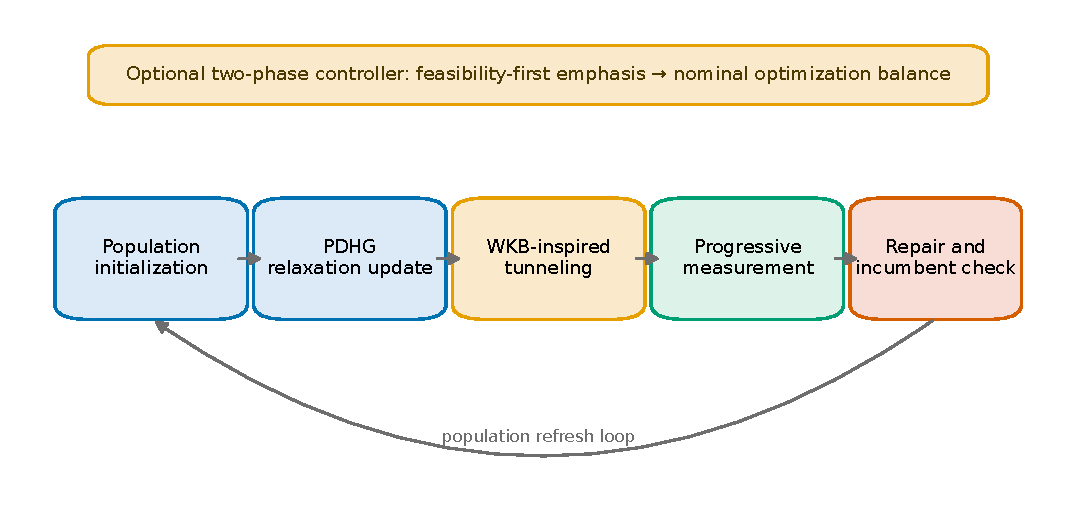
\includegraphics[width=0.82\textwidth]{figures/framework_overview_nature.pdf}
    \caption{Overview of the HP-PDHG workflow. The figure highlights the information flow from relaxation search to incumbent update and clarifies the distinct roles of population diversification, barrier-aware perturbation, integrality projection, and feasibility-preserving repair.}
    \label{fig:framework}
\end{figure}

We score tentative states with a penalized energy that augments the linear objective by terms for primal infeasibility and integrality residual:
\begin{equation}
E(x) = c^T x + \rho_c \sum_{i=1}^{m} \max(0, a_i^T x - b_i)^2 + \rho_i \sum_{j \in \mathcal{I}} \text{dist}(x_j, \mathbb{Z})^2.
\label{eq:energy}
\end{equation}
The energy is not the reported optimization objective; rather, it serves as a guide for accepting or rejecting tentative moves. Candidates are ultimately evaluated in the original MIP objective and must pass explicit feasibility checks before they can become incumbents.

\subsection{Population-Based PDHG Backbone}
\label{subsec:pop_pdhg}

Let $\mathcal{P} = \{(x^{(1)}, y^{(1)}), \ldots, (x^{(K)}, y^{(K)})\}$ denote the population of primal-dual states. Each member follows the PDHG updates
\begin{align}
    x^{t+1,(k)} &= \Pi_{[l,u]}\left(x^{t,(k)} - \tau(c + A^T y^{t,(k)})\right), \\
    \bar{x}^{t+1,(k)} &= 2x^{t+1,(k)} - x^{t,(k)}, \\
    y^{t+1,(k)} &= \Pi_{\mathbb{R}^m_+}\left(y^{t,(k)} + \sigma(A\bar{x}^{t+1,(k)} - b)\right),
\end{align}
with shared step sizes chosen from a spectral norm estimate of $A$. The purpose of the population is not merely parallelism. Different members occupy different attraction basins of the relaxation, which raises the chance that at least one candidate approaches an $\epsilon$-feasible region even when individual trajectories are initialization-sensitive.

In implementation, we initialize the population with mild but deliberate diversity. Some members start near the origin or a clipped zero vector, while others receive perturbations of different magnitudes. Elite candidates are tracked for proposal guidance and incumbent selection, but the population is not collapsed to a single path. This design lets the method exploit the stability of PDHG without suffering the brittleness of a single-trajectory heuristic.

\subsection{Feasibility-First Two-Phase Control}
\label{subsec:two_phase}

The current implementation also exposes an optional two-phase schedule that changes the relative emphasis of feasibility and objective improvement during a run. Let $T$ be the iteration budget and let
\begin{equation}
T_1 = \lfloor \eta T \rfloor,
\qquad
\omega_t =
\begin{cases}
\omega_{\mathrm{feas}}, & t \leq T_1, \\
1, & t > T_1,
\end{cases}
\label{eq:two_phase}
\end{equation}
where $\eta \in (0,1)$ is the feasibility-phase ratio and $\omega_{\mathrm{feas}} > 1$ is a constraint-emphasis multiplier. In Phase~1, the solver prioritizes feasibility by amplifying the dual response after the PDHG update and by applying measurement more frequently. In Phase~2, the dual weight is reset to one and the algorithm returns to its nominal balance between objective reduction and constraint satisfaction.

Operationally, the dual state after a PDHG step is scaled by $\omega_t$ and clipped in implementation to avoid numerical overflow. The projection interval is also shortened in the feasibility phase,
\begin{equation}
\tau_{\mathrm{measure}}^{(1)} = \max\!\left(20, \left\lfloor \frac{\tau_{\mathrm{measure}}}{2} \right\rfloor \right),
\label{eq:phase_measure}
\end{equation}
and restored to $\tau_{\mathrm{measure}}$ once Phase~2 begins. This mechanism does not introduce a new search operator. Rather, it changes when the existing PDHG, integrality-projection, and repair operators are emphasized. We include it here because it is part of the current solver interface, although the benchmark, ablation, and sensitivity results in this paper primarily analyze the enhanced repair and barrier-aware perturbation path rather than isolating the two-phase controller itself.

\subsection{Barrier-Aware Non-Local Perturbation}
\label{subsec:tunneling}

\subsubsection{Design Motivation}

The Wentzel-Kramers-Brillouin approximation in quantum mechanics describes the probability that a particle crosses a potential barrier without acquiring enough classical energy to go over it. In its canonical one-dimensional form, the tunneling probability decays exponentially with an action term that depends on both barrier height and barrier width. We borrow this width-sensitive intuition only as a design cue. In the optimization setting, infeasible regions can act as thin walls separating promising basins, so a barrier-aware acceptance rule can be more informative than either purely local search or indiscriminate random restarts.

\subsubsection{Optimization Analog}

We translate this intuition into the acceptance model
\begin{equation}
P_{\text{tunnel}}(x \to x') = \exp\left(-\Gamma \|x - x'\| \sqrt{\max(E(x') - E(x), 0)}\right),
\label{eq:tunnel_prob}
\end{equation}
where $\Gamma > 0$ controls exploration intensity and $E$ is the penalized energy from \eqref{eq:energy}. The rule discourages large uphill moves but does not forbid them. Thin or low barriers can still be crossed with appreciable probability, which is the intended algorithmic analogue of a tunneling-style barrier-crossing move.

\begin{figure}[htbp]
    \centering
    \begin{subfigure}[b]{0.47\textwidth}
        \centering
        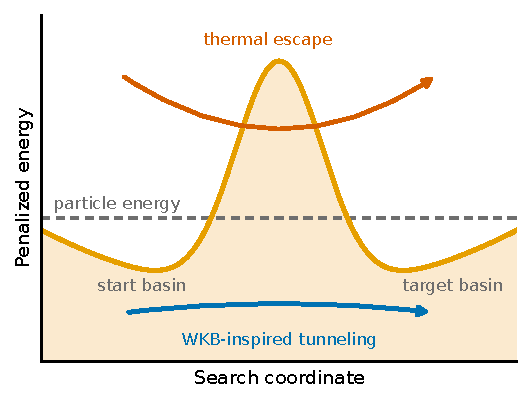
\includegraphics[width=\textwidth]{figures/tunneling_barrier_nature.pdf}
        \caption{Thermal escape versus tunneling-style escape.}
        \label{fig:tunnel_barrier}
    \end{subfigure}
    \hfill
    \begin{subfigure}[b]{0.47\textwidth}
        \centering
        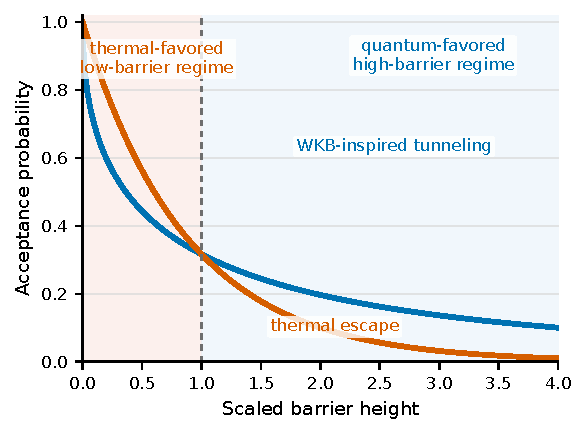
\includegraphics[width=\textwidth]{figures/tunneling_probability_nature.pdf}
        \caption{Acceptance profiles across increasing barrier height under a fixed effective jump width.}
        \label{fig:tunnel_probability}
    \end{subfigure}
    \caption{Conceptual schematic for the barrier-aware perturbation used in HP-PDHG. The right panel shows a one-dimensional slice in which the effective jump width and proportionality constants are absorbed into the horizontal scaling, so thermal escape decays as $\exp(-\beta h)$ while the WKB-inspired profile decays as $\exp(-\gamma \sqrt{h})$. The figure is intended as design intuition for the acceptance rule rather than as a claim of physical simulation.}
    \label{fig:tunneling_mechanism}
\end{figure}

Figure~\ref{fig:tunneling_mechanism} makes this distinction explicit. The left panel highlights the qualitative difference between surmounting a barrier and passing through it, while the right panel visualizes the fixed-width slice implied by \eqref{eq:tunnel_prob}. In the plotted schematic we set the two proportionality constants equal, so the crossover occurs at unit scaled barrier height. In the full algorithm, acceptance also depends on the proposal distance $\|x'-x\|$; the plotted curves therefore capture the correct functional trend rather than every degree of freedom in the multivariate rule.

\subsubsection{Multi-Scale L\'{e}vy Proposals}

When a non-local perturbation is triggered, proposals are generated from a mixture of proposal modes. History-guided moves interpolate toward elite incumbents, population-guided moves exploit directions suggested by the current ensemble, and random L\'{e}vy proposals provide heavy-tailed exploration that can jump between distant basins. The heavy-tailed component is especially important because Gaussian perturbations are too local to mimic barrier-crossing behavior in difficult feasibility landscapes. In practice, the proposal family is clipped to the bound box before acceptance is evaluated.

\subsection{Progressive Integrality Projection}
\label{subsec:measurement}

\subsubsection{Motivation}

Immediate rounding is often harmful in MIP because many coordinates are forced onto the integer lattice at once, often creating large primal violations. We therefore use progressive integrality projection, which lets the algorithm continue to benefit from the smooth geometry of the relaxation while gradually increasing discrete pressure.

\subsubsection{Cosine-Annealed Schedule}

The projection strength is controlled by
\begin{equation}
\lambda_t = \lambda_{\min} + \frac{\lambda_{\max} - \lambda_{\min}}{2}\left(1 - \cos\left(\pi \frac{t}{T}\right)\right),
\label{eq:measurement_schedule}
\end{equation}
where $T$ is the iteration budget. Early iterations have small $\lambda_t$, so the dynamics remain close to the continuous relaxation. Later iterations move $\lambda_t$ toward one, thereby shifting the search from exploration to discrete commitment.

\subsubsection{Soft Rounding Operator}

For each integer-constrained coordinate, we apply the soft-rounding map
\begin{equation}
\tilde{x}_j =
\begin{cases}
(1-\lambda_t)x_j + \lambda_t \operatorname{round}(x_j), & j \in \mathcal{I}, \\
x_j, & j \notin \mathcal{I}.
\end{cases}
\label{eq:soft_measurement}
\end{equation}
By Theorem~\ref{thm:measurement}, this operator contracts the integrality residual by a factor of $(1-\lambda_t)$ on every projected coordinate. The projection stage is therefore analytically interpretable rather than purely heuristic: it systematically reduces non-integrality while still leaving room for the repair stage to absorb small constraint violations.

\subsection{Feasibility-Aware Repair}
\label{subsec:repair}

Candidates generated by non-local perturbation or integrality projection are not accepted directly. Instead, they pass through a mixed-integer repair procedure that mirrors the current mainline implementation. The first stage clips variables to the bound box and rapidly repairs obvious binary violations by greedy flips. The second stage applies gradient-projection steps to the positive-part constraint residual, reprojects to the bounds, and rounds general integer coordinates after each candidate update. If this projected descent stalls, a local coordinate-descent pass is used as a fallback on the integer variables. A simpler projection-only repair routine is also available in the codebase, but the ablation and sensitivity studies reported here use the enhanced mixed-integer repair path. Repair is intentionally conservative: a candidate is promoted only if the final result satisfies the linear constraints, bounds, and integrality tests and remains competitive in objective value. This policy lets the algorithm explore aggressively at the candidate level while preserving a reliable incumbent set.

\subsection{Complete Algorithm}
\label{subsec:algorithm}

Algorithm~\ref{alg:quantum_pop_pdhg} summarizes the full procedure.

\begin{algorithm}[htbp]
\caption{HP-PDHG algorithmic workflow.}
\label{alg:quantum_pop_pdhg}
\begin{algorithmic}[1]
\REQUIRE Constraint matrix $A$, right-hand side $b$, objective $c$, bounds $l,u$, integer set $\mathcal{I}$, population size $K$, maximum iterations $T$, feasibility ratio $\eta$, feasibility weight $\omega_{\mathrm{feas}}$
\STATE Initialize population $\{(x^{(k)}, y^{(k)})\}_{k=1}^K$
\STATE Initialize best feasible solution $x^* \leftarrow \varnothing$
\STATE $T_1 \leftarrow \lfloor \eta T \rfloor$, $\omega \leftarrow \omega_{\mathrm{feas}}$
\FOR{$t = 1$ to $T$}
    \IF{$t = T_1 + 1$}
        \STATE $\omega \leftarrow 1$
    \ENDIF
    \FOR{$k = 1$ to $K$}
        \STATE Update $(x^{(k)}, y^{(k)})$ by one PDHG step
        \IF{$t \leq T_1$}
            \STATE Scale the dual state by $\omega$
            \STATE $\tau_{\text{measure}}^{(t)} \leftarrow \max(20,\lfloor \tau_{\text{measure}}/2 \rfloor)$
        \ELSE
            \STATE $\tau_{\text{measure}}^{(t)} \leftarrow \tau_{\text{measure}}$
        \ENDIF
        \IF{mod$(t, \tau_{\text{tunnel}}) = 0$}
            \STATE Sample tunneling proposal $x'$
            \IF{$x'$ is accepted by \eqref{eq:tunnel_prob}}
                \STATE $x^{(k)} \leftarrow x'$
            \ENDIF
        \ENDIF
        \IF{mod$(t, \tau_{\text{measure}}^{(t)}) = 0$}
            \STATE $\tilde{x} \leftarrow$ Soft\_Round$(x^{(k)}, \lambda_t)$
            \STATE $x^{(k)} \leftarrow$ Feasibility\_Repair$(\tilde{x})$
        \ENDIF
        \IF{$x^{(k)}$ is feasible and improves the incumbent}
            \STATE $x^* \leftarrow x^{(k)}$
        \ENDIF
    \ENDFOR
\ENDFOR
\RETURN $x^*$
\end{algorithmic}
\end{algorithm}

The practical interpretation of the algorithm is straightforward. PDHG provides a stable large-scale relaxation solver, the barrier-aware perturbation prevents the population from remaining confined to a single basin, integrality projection gradually contracts fractional coordinates, and repair plus incumbent screening preserves feasibility. The method is therefore not a collection of loosely connected heuristics, but a coordinated pipeline in which each component addresses a specific obstacle in moving from relaxation quality to integer-feasible incumbents.


\section{Experimental Results}
\label{sec:experiments}
\subsection{Experimental Setup}
\label{subsec:setup}

\subsubsection{Layered benchmark protocol}

The empirical study is organized in three layers because the paper addresses three questions. The first question is \emph{whether the proposed pipeline can reliably convert a strong fractional trajectory into a strictly feasible mixed-integer incumbent}. For that purpose we retain the four-instance audited benchmark used throughout Plan~1: p0033, p0201, p0282, and knapsack\_50. These instances are small enough that every candidate solution can be inspected carefully, yet still diverse enough to expose the core feasibility transition studied in the paper.

The second question is \emph{whether the same architecture remains competitive once we move from illustrative audited cases to a standardized MIPLIB 2017 benchmark protocol}. To answer that question, we parsed the official MIPLIB 2017 benchmark-v2 test set and the official v36 \texttt{.solu} reference file, then filtered instances by predeclared structural rules rather than by ex post performance: known official reference value, 100--3000 variables, 50--2500 constraints, at least 20 integer variables, integer ratio at least 0.30, and at most 60{,}000 nonzeros. These rules yielded a 29-instance candidate pool. From that pool we selected twelve size-diverse instances by a deterministic stratified procedure and copied only those files into the local \texttt{Plan 1/data/miplib2017\_sec} directory. The resulting official subset spans 274--2500 variables and 233--2107 constraints, with a median integer ratio above 0.93; instance-level names and sizes are reported in Table~\ref{tab:extended_benchmark}.

Finally, to position the method against widely used intelligent population heuristics, we extracted the six smallest instances from the official subset and ran an additional representative comparison against GA, DE, SHADE, and SL-PSO, together with the archived implementation variants Standard Pop-PDHG and Quantum Pop-PDHG. This third layer is not used to replace the fully audited four-instance feasibility benchmark; rather, it tests whether the proposed hybrid feasibility-recovery architecture occupies a competitive position relative to established population-based baselines when all methods are evaluated under the same repaired feasibility audit. To keep the data chain auditable, the raw result files retain the archived implementation labels, while the manuscript refers to them conceptually as the baseline and hybrid variants.

\subsubsection{Baselines, repeated runs, and audited metrics}

Our primary controlled comparator remains \emph{Standard Pop-PDHG}, obtained by disabling the barrier-crossing and progressive integrality-projection enhancements while preserving the common population backbone, PDHG updates, and repair infrastructure. Throughout the narrative below, we refer to the proposed method as HP-PDHG; in the stored implementation and result tables, the same solver appears under the legacy name \emph{Quantum Pop-PDHG}. Gurobi~13.0.1 \cite{gurobi2024} provides the exact-solver reference. For the official MIPLIB 2017 extension we use the official v36 \texttt{.solu} file as the authoritative objective reference, while a 60-second Gurobi run is retained as an additional local sanity check.

For the population-based comparison we evaluate four broader metaheuristics: a real-coded genetic algorithm, DE, SHADE, and SL-PSO \cite{storn1997de,tanabe2013shade,cheng2015slpso}. To make the comparison fair, these baselines are not judged on raw penalized fitness alone. Instead, after each run we pass the incumbent through the same audited feasibility-repair layer used by the proposed method, then re-evaluate it against the \emph{original} constraint senses, bound constraints, and integrality conditions. This common post-processing step is important because otherwise different solvers would be compared through incompatible definitions of constraint satisfaction.

Every reported value in the paper therefore corresponds to one of three audited quantities: objective value, maximum primal violation with respect to the original MPS model, and feasibility status after explicit rechecking of integrality and bounds. For the four-instance audited benchmark we also report absolute percentage gap to the exact Gurobi optimum, and we additionally rerun that benchmark over 20 seeds to quantify robustness. For the official benchmark extension and the population-based baseline study, the main performance variable is the final maximum violation, because many runs remain infeasible under the fixed budget and any ``objective'' attached to an infeasible point is only diagnostic. The official extension uses five random seeds per solver, and the representative population-based baseline study uses the same five-seed protocol.

\subsubsection{Implementation, hardware, and reproducibility}

All experiments were executed on a MacBook Pro with Apple M4 Pro CPU (12 cores) and 24\,GB unified memory using Python~3.13, NumPy, SciPy, and Gurobi. The key correction relative to earlier project iterations is that the final experimental chain no longer relies on permissive feasibility checks. Earlier legacy scripts occasionally hard-coded optimal values, ignored original constraint senses, or failed to recompute the objective after repair. The audited Plan~1 pipeline corrects those issues. In particular, the final benchmark scripts use the original MPS files, the official \texttt{.solu} references for MIPLIB 2017, original bound data, and explicit post-repair verification. For a paper whose central claim is feasibility recovery rather than relaxed objective quality, that audit is not a cosmetic detail; it is part of the contribution.

\subsection{Audited Feasibility-Recovery Benchmark}
\label{subsec:main_results}

Table~\ref{tab:main_results} reports the main audited benchmark. The pattern is unambiguous. The baseline Pop-PDHG variant drives the relaxation to attractive objective regions on all four instances, but it remains infeasible after explicit rechecking. By contrast, HP-PDHG recovers strict feasibility on all four. It matches the Gurobi optimum on p0033, reaches a feasible incumbent within 2.21\% of optimum on p0201, crosses the p0282 near-feasibility barrier with only a 0.16\% gap, and returns a feasible solution within 0.54\% of optimum on knapsack\_50.

\begin{table}[htbp]
\centering
\caption{Audited four-instance feasibility-recovery benchmark. Gaps are absolute percentages relative to the Gurobi optimum. For infeasible solvers, the objective is diagnostic only and does not constitute a valid primal bound, which is why feasibility status remains the primary operational criterion.}
\label{tab:main_results}
\small
\resizebox{\textwidth}{!}{%
\begin{tabular}{llccccc}
\toprule
\textbf{Instance} & \textbf{Solver} & \textbf{Objective} & \textbf{Abs.\ gap (\%)} & \textbf{Max violation} & \textbf{Time (s)} & \textbf{Feasible} \\
\midrule
\multirow{3}{*}{p0033}
& Gurobi & -68.0000 & -- & 0 & 0.004 & Yes \\
& Baseline Pop-PDHG & -86.0000 & 26.47 & 1.4409 & 0.369 & No \\
& \textbf{HP-PDHG} & \textbf{-68.0000} & \textbf{0.00} & \textbf{0} & \textbf{0.473} & \textbf{Yes} \\
\midrule
\multirow{3}{*}{p0201}
& Gurobi & -226.0000 & -- & 0 & 0.007 & Yes \\
& Baseline Pop-PDHG & -239.0000 & 5.75 & 1.8988 & 2.080 & No \\
& \textbf{HP-PDHG} & \textbf{-221.0000} & \textbf{2.21} & \textbf{0} & \textbf{2.707} & \textbf{Yes} \\
\midrule
\multirow{3}{*}{p0282}
& Gurobi & -7899.4132 & -- & 0 & 0.013 & Yes \\
& Baseline Pop-PDHG & -7888.3187 & 0.14 & 0.0805 & 2.956 & No \\
& \textbf{HP-PDHG} & \textbf{-7887.0719} & \textbf{0.16} & \textbf{$9.87\times10^{-7}$} & \textbf{4.234} & \textbf{Yes} \\
\midrule
\multirow{3}{*}{knapsack\_50}
& Gurobi & -2051.0000 & -- & 0 & 0.001 & Yes \\
& Baseline Pop-PDHG & -2076.0000 & 1.22 & 3.4000 & 0.526 & No \\
& \textbf{HP-PDHG} & \textbf{-2040.0000} & \textbf{0.54} & \textbf{0} & \textbf{0.640} & \textbf{Yes} \\
\bottomrule
\end{tabular}%
}
\end{table}

Two details are worth emphasizing. First, the objective values of the infeasible baseline Pop-PDHG rows are often numerically attractive, but they are scientifically secondary because they do not correspond to valid incumbents. The p0282 case is especially instructive: the baseline variant appears superficially competitive on objective value, yet it still violates the original model by $8.05\times 10^{-2}$. HP-PDHG sacrifices only a small additional amount of objective quality in exchange for verified feasibility. Second, the p0033 row shows that the proposed pipeline is not merely a ``repair to any feasible point'' strategy. When the instance geometry is favorable, the method can recover feasibility without paying an objective premium at all.

The same message survives aggressive repetition. We reran the four audited instances over 20 seeds per solver, yielding 80 paired runs. HP-PDHG produced a verified feasible incumbent in all 80 runs, whereas the baseline Pop-PDHG variant produced none. The exact paired sign test on discordant feasibility outcomes gives $p=8.27\times10^{-25}$, and the paired Wilcoxon test on audited primal violations gives $p=2.75\times10^{-15}$. These repeated-run results matter because they convert Table~\ref{tab:main_results} from a visually compelling but small benchmark into a statistically overwhelming robustness result for the specific feasibility-recovery claim made in the paper.

Figure~\ref{fig:p0282_tradeoff} visualizes the p0282 mechanism from another angle. The baseline variant sits in a low-objective but still infeasible basin. The hybrid variant moves slightly away from that basin in objective space but crosses the final feasibility barrier. In other words, the contribution of the method is not better local optimization on the relaxation; it is a more reliable transition from a strong fractional point to an admissible integer point.

\begin{figure}[htbp]
\centering
\begin{subfigure}[b]{0.31\textwidth}
    \centering
    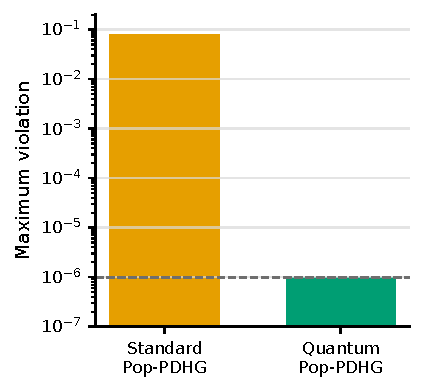
\includegraphics[width=\textwidth]{figures/p0282_feasibility_nature.pdf}
    \caption{Maximum violation}
\end{subfigure}
\hfill
\begin{subfigure}[b]{0.31\textwidth}
    \centering
    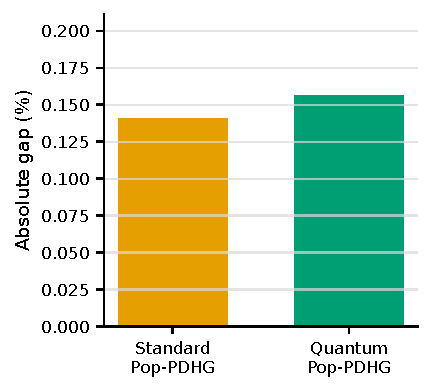
\includegraphics[width=\textwidth]{figures/p0282_gap_nature.pdf}
    \caption{Absolute objective gap}
\end{subfigure}
\hfill
\begin{subfigure}[b]{0.31\textwidth}
    \centering
    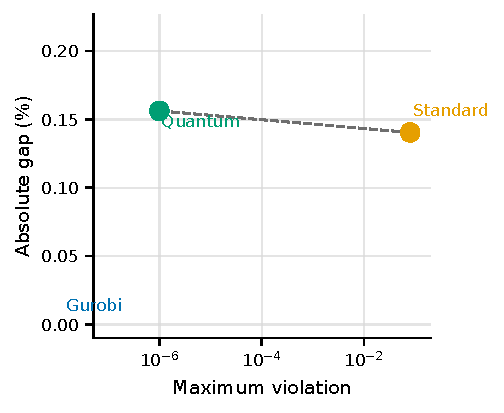
\includegraphics[width=\textwidth]{figures/p0282_tradeoff_nature.pdf}
    \caption{Feasibility--gap trade-off}
\end{subfigure}
\caption{Audited behavior on p0282. The baseline variant reaches a strong but invalid near-feasible point, whereas HP-PDHG crosses the final feasibility barrier with only a modest additional objective sacrifice, illustrating the practical value of converting a good fractional plan into an admissible decision.}
\label{fig:p0282_tradeoff}
\end{figure}

\subsection{Official MIPLIB 2017 Extension}
\label{subsec:extended_official}

The four-instance audited benchmark establishes that the method can perform the central feasibility transition. The next question is whether the same behavior persists on a standardized official benchmark subset selected without looking at solver outcomes. Table~\ref{tab:extended_benchmark} addresses that question on the twelve-instance MIPLIB 2017 extension.

\begin{table}[htbp]
\centering
\caption{Official MIPLIB 2017 extension under a fixed budget of 1000 iterations and five random seeds. Reported violations are per-instance means after audited repair and rechecking, so the table measures how effectively each method reduces residual infeasibility when full closure is still difficult.}
\label{tab:extended_benchmark}
\small
\resizebox{\textwidth}{!}{%
\begin{tabular}{lcccccc}
\toprule
\textbf{Instance} & \textbf{$n$} & \textbf{$m$} & \textbf{Integer ratio} & \textbf{Baseline mean violation} & \textbf{HP-PDHG mean violation} & \textbf{Reduction (\%)} \\
\midrule
glass4 & 322 & 396 & 0.94 & $3.00\times10^{5}$ & $3.00\times10^{5}$ & 0.0 \\
neos-3046615-murg & 274 & 498 & 0.93 & 53.60 & 20.00 & 62.7 \\
neos-2657525-crna & 524 & 342 & 1.00 & $5.71\times10^{3}$ & $2.65\times10^{3}$ & 53.6 \\
ic97\_potential & 728 & 1046 & 0.72 & 33.92 & 34.94 & -3.0 \\
cod105 & 1024 & 1024 & 1.00 & 0.00 & 0.00 & 0.0 \\
gmu-35-40 & 1205 & 424 & 1.00 & 19.52 & 13.54 & 30.6 \\
neos-4954672-berkel & 1533 & 1848 & 0.41 & $7.29\times10^{3}$ & $7.21\times10^{3}$ & 1.0 \\
mcsched & 1747 & 2107 & 1.00 & 934.80 & 1069.48 & -14.4 \\
gmu-35-50 & 1919 & 435 & 1.00 & 14.36 & 10.30 & 28.3 \\
50v-10 & 2013 & 233 & 0.82 & 148.14 & 136.11 & 8.1 \\
p200x1188c & 2376 & 1388 & 0.50 & $2.58\times10^{3}$ & $4.71\times10^{2}$ & 81.8 \\
beasleyC3 & 2500 & 1750 & 0.50 & 21.72 & 15.82 & 27.2 \\
\bottomrule
\end{tabular}%
}
\end{table}

Several points emerge from this table. First, the official extension is markedly harder than the audited four-instance benchmark. Even with 1000 iterations and five seeds, the only instance solved to strict feasibility by both methods in all runs is cod105. This is useful information rather than a failure of reporting. It shows that once the benchmark is broadened, the scientific question shifts from ``can the method ever cross the feasibility barrier?'' to ``does the proposed mechanism reduce the residual distance to feasibility more effectively than the baseline under a fixed computation budget?'' That is precisely why the maximum violation becomes the primary metric in the extension.

Second, the added hybrid mechanisms now produce a broader and statistically stronger directional advantage on the official subset. HP-PDHG lowers the mean audited violation on eight of the twelve instances, ties on two, and loses on two; the median per-instance change is a 27.2\% reduction. The strongest improvements occur on p200x1188c (81.8\%), neos-3046615-murg (62.7\%), neos-2657525-crna (53.6\%), gmu-35-40 (30.6\%), gmu-35-50 (28.3\%), and beasleyC3 (27.2\%). The mixed cases remain informative: ic97\_potential is a near-tie with a slight disadvantage for HP-PDHG, and mcsched remains a genuine counterexample.

Third, the extension provides a more favorable but still honest calibration of the method's current maturity. The paired Wilcoxon test on per-instance mean violations now favors HP-PDHG at the 5\% level ($p=0.032$). We therefore have stronger evidence than before that the proposed architecture reduces distance to feasibility on official instances under a fixed budget. At the same time, the interpretation should remain disciplined: two instances are exact ties, glass4 is a pathological outlier, and the strict-feasibility count does not yet show broad large-scale closure beyond cod105. The contribution supported by these data is therefore \emph{improved official-benchmark feasibility reduction}, not universal official-benchmark dominance.

These trends are summarized visually in Figure~\ref{fig:sec_official}. The figure should be read as an extension study, not as the central proof of feasibility recovery.

\begin{figure}[htbp]
\centering
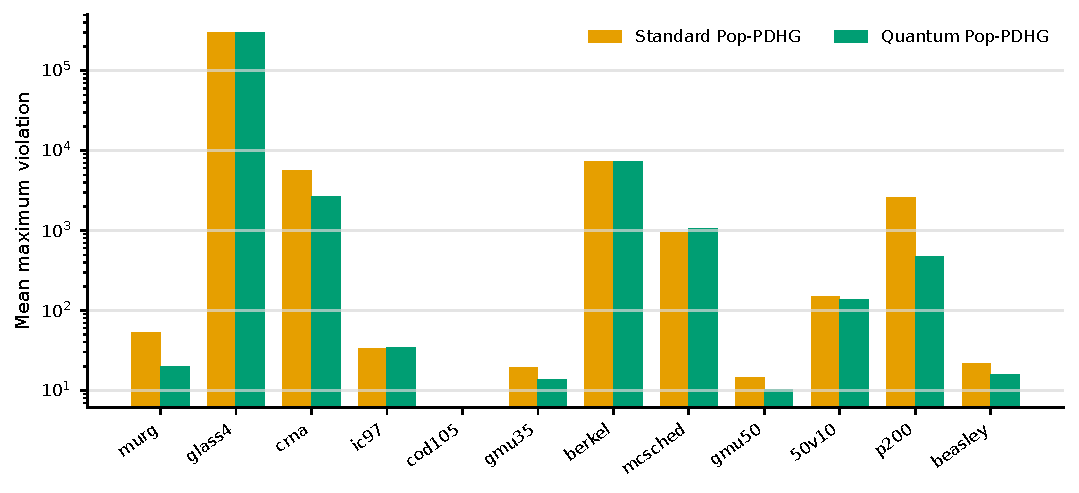
\includegraphics[width=0.92\textwidth]{figures/sec_official_benchmark_nature.pdf}
\caption{Official MIPLIB 2017 extension. Bars report mean audited maximum violation over five seeds. HP-PDHG improves eight instances, ties two, and loses two under a fixed 1000-iteration budget, which supports the view that the method is most useful as a feasibility-reduction module on harder instances.}
\label{fig:sec_official}
\end{figure}

\subsection{Comparison with Population-Based Metaheuristics}
\label{subsec:sec_baselines}

The population-based baseline study asks a different but complementary question: if we ignore exact proof of optimality and compare only population-based heuristics under the same repaired feasibility audit, where does HP-PDHG sit relative to standard intelligent search methods? Table~\ref{tab:sec_rank_table} summarizes the answer on the six smallest official instances from the 12-instance official subset, using per-instance mean audited violation and Friedman ranks.

\begin{table}[htbp]
\centering
\caption{Average Friedman ranks on the six-instance representative population-based baseline study. Lower is better. The table is intended to show comparative placement among intelligent heuristics rather than universal pairwise dominance.}
\label{tab:sec_rank_table}
\small
\begin{tabular}{lcc}
\toprule
\textbf{Solver} & \textbf{Average rank} & \textbf{Mean violation} \\
\midrule
HP-PDHG & \textbf{1.75} & $5.05\times10^{4}$ \\
SHADE & 2.67 & $1.09\times10^{6}$ \\
Baseline Pop-PDHG & 3.08 & $5.10\times10^{4}$ \\
SL-PSO & 4.00 & $1.99\times10^{5}$ \\
DE & 4.67 & $6.55\times10^{6}$ \\
GA & 4.83 & $1.59\times10^{6}$ \\
\bottomrule
\end{tabular}
\end{table}

The first observation is encouraging for the proposed method: HP-PDHG attains the best average rank (1.75), ahead of SHADE, the baseline Pop-PDHG variant, SL-PSO, DE, and GA. The second observation is equally important: this leadership is not uniform across all instances. On neos-3046615-murg and gmu-35-40, HP-PDHG is clearly strongest. On glass4 and cod105, the two PDHG variants are tied at the best observed violation. On neos-2657525-crna, HP-PDHG is near-best but SHADE performs slightly better. On ic97\_potential, the baseline variant is marginally better than the hybrid one. This is exactly the kind of pattern a credible hybrid heuristic should produce: strong average placement and identifiable strengths, but not artificial claims of instance-by-instance invincibility.

This mixture of wins, ties, and close second-place finishes is visible in Figures~\ref{fig:sec_ranks} and~\ref{fig:sec_heatmap}. The rank plot captures the overall pattern across instances; the heatmap shows that the proposed method is not simply globally dominant, but rather occupies a competitive niche. It tends to be strongest when relaxation information remains useful and the feasibility transition is the real bottleneck. From a scientific perspective, this is exactly the kind of evidence a hybrid heuristic should provide: not the fantasy of universal dominance, but a clear statement of where the method fits among established intelligent baselines.

The nonparametric tests tell the same story in a more disciplined way. The overall Friedman test is now significant at the 5\% level ($p=0.016$), which supports the claim that the six solvers are not statistically indistinguishable on this representative subset. However, the Holm-adjusted pairwise Wilcoxon tests remain conservative, so the correct interpretation is \emph{significant overall ordering with cautious post-hoc claims}, not pairwise universal superiority. Within that boundary, HP-PDHG still emerges as the best-ranked method on average.

\begin{figure}[htbp]
\centering
\begin{subfigure}[b]{0.43\textwidth}
    \centering
    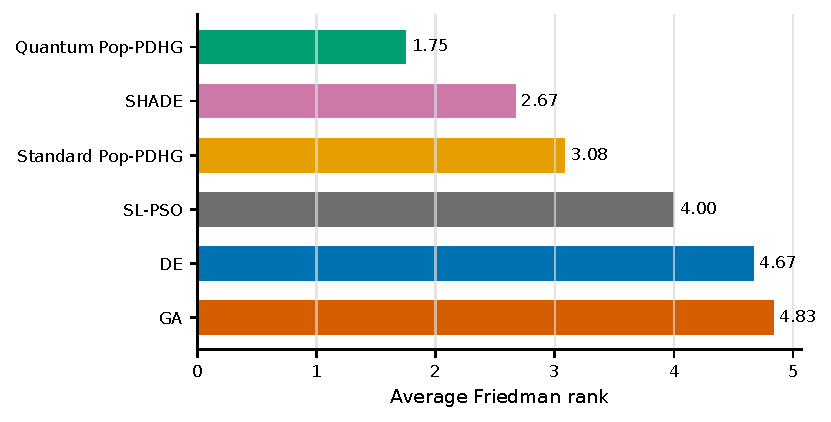
\includegraphics[width=\textwidth]{figures/sec_metaheuristic_ranks_nature.pdf}
    \caption{Average ranks}
    \label{fig:sec_ranks}
\end{subfigure}
\hfill
\begin{subfigure}[b]{0.53\textwidth}
    \centering
    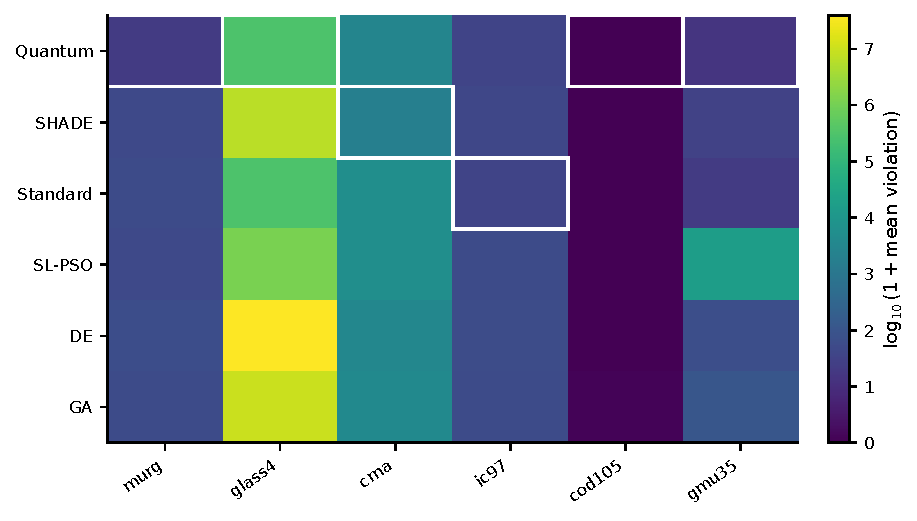
\includegraphics[width=\textwidth]{figures/sec_metaheuristic_heatmap_nature.pdf}
    \caption{Per-instance violation heatmap}
    \label{fig:sec_heatmap}
\end{subfigure}
\caption{Representative comparison against population-based intelligent baselines. The archived solver variant labeled Quantum Pop-PDHG, corresponding to HP-PDHG in the manuscript, attains the best average rank, while the heatmap clarifies that its advantage is instance dependent rather than universal. White outlines indicate the best solver on each instance and highlight the heterogeneity that motivates hybrid or portfolio use.}
\label{fig:sec_meta}
\end{figure}

\subsection{Ablation of the Added Mechanisms}
\label{subsec:ablation}

The current implementation includes several modules that were added during the later development stages of Plan~1, including the second-stage feasibility-first controller, the projection-based repair path, and the progressive integrality-projection schedule. The ablation study isolates the most practically important components. Table~\ref{tab:ablation} aggregates the corrected ablation results across the four-instance audited benchmark.

\begin{table}[htbp]
\centering
\caption{Aggregated ablation results on the four-instance audited benchmark. ``Feasible instances'' counts how many of the four instances end in verified strict feasibility. Mean feasible gap is reported only over successful runs, allowing the contribution of each module to be interpreted separately.}
\label{tab:ablation}
\small
\resizebox{\textwidth}{!}{%
\begin{tabular}{lcccc}
\toprule
\textbf{Configuration} & \textbf{Feasible instances} & \textbf{Mean feasible gap (\%)} & \textbf{Mean runtime (s)} & \textbf{Mean tunnel success rate (\%)} \\
\midrule
Base Pop-PDHG & 0/4 & -- & 1.98 & 0.0 \\
+ Barrier-Aware Perturbation & 0/4 & -- & 1.98 & 28.5 \\
+ Progressive Projection & 4/4 & 0.727 & 2.51 & 0.0 \\
+ HMC Dynamics & 0/4 & -- & 1.98 & 0.0 \\
Full HP-PDHG & 4/4 & 0.726 & 2.51 & 42.6 \\
\bottomrule
\end{tabular}
}
\end{table}

The qualitative message of Table~\ref{tab:ablation} is stronger than any single row. The barrier-aware perturbation alone changes exploration statistics and produces accepted non-local moves, but it does not by itself recover strict feasibility. HMC dynamics, in the present implementation, also do not change that conclusion. Progressive projection is the turning point: once staged integrality enforcement is turned on, the solver crosses from attractive but infeasible trajectories to verified feasible incumbents on all four audited cases. The full method then preserves that feasibility profile while increasing the accepted-jump rate, which supports the interpretation that the non-local perturbation is \emph{complementary} rather than \emph{sufficient}. It helps diversify search, but the actual feasibility transition is carried primarily by projection and repair.

\subsection{Parameter Sensitivity}
\label{subsec:sensitivity}

We additionally reran the parameter-sensitivity study on the corrected code path, for a total of 390 audited runs. The purpose of this study is not exhaustive hyperparameter tuning; it is to determine whether the proposed method depends on a narrow and fragile set of parameter values. The answer is encouraging. Across the easy audited instances, the method operates on a broad stable plateau rather than a knife-edge optimum.

Figure~\ref{fig:sensitivity} summarizes two representative trends. Increasing the tunnel interval from 25 toward 100--200 typically improves the quality of accepted jumps because the population has more time to reshape the relaxation trajectory between non-local transitions. At the same time, larger populations increase runtime roughly monotonically, but they do not produce a corresponding monotonic gain in final solution quality on the easy audited instances. This is exactly the sensitivity pattern one would hope for in a practical heuristic: the parameters matter, but the mainline configuration is not rescued by a single exceptional setting.

\begin{figure}[htbp]
\centering
\begin{subfigure}[b]{0.46\textwidth}
    \centering
    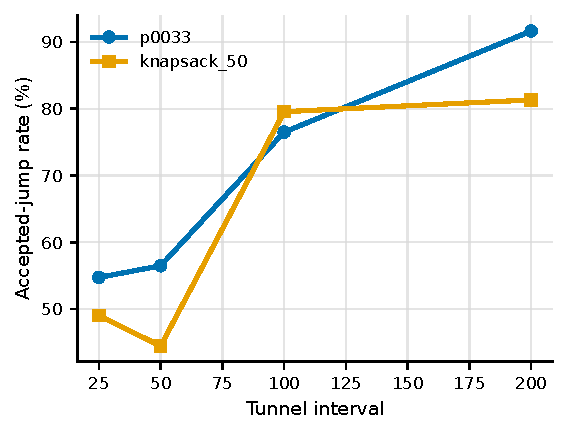
\includegraphics[width=\textwidth]{figures/sensitivity_tunnel_interval_nature.pdf}
    \caption{Tunnel interval}
\end{subfigure}
\hfill
\begin{subfigure}[b]{0.46\textwidth}
    \centering
    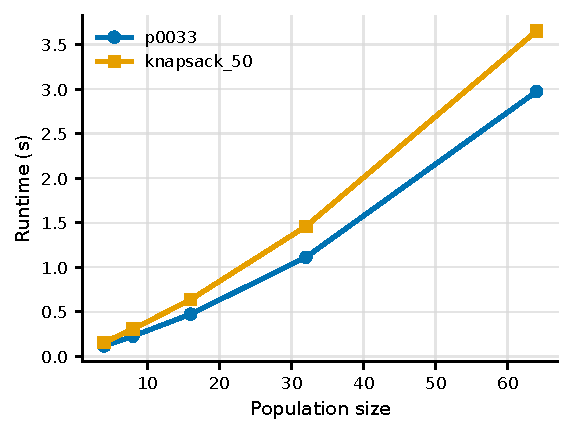
\includegraphics[width=\textwidth]{figures/sensitivity_population_size_nature.pdf}
    \caption{Population size}
\end{subfigure}
\caption{Representative sensitivity trends from the corrected 390-run study. The method exhibits a broad practical plateau rather than a narrow hyperparameter optimum, which is encouraging for low-tuning deployment.}
\label{fig:sensitivity}
\end{figure}

It is also worth clarifying what the sensitivity study does and does not show. Because it is run on the four audited feasibility-recovery instances, it is primarily a \emph{stability} analysis of the mainline implementation rather than a substitute for the official MIPLIB 2017 extension. The two studies therefore play different roles in the paper. The sensitivity analysis shows that the audited feasibility-recovery result is not brittle; the official extension shows how far the same mechanism generalizes once the benchmark becomes materially harder.

\subsection{Discussion}
\label{subsec:discussion}

Taken together, the experiments support a precise interpretation of the method. HP-PDHG is already convincing as a \emph{feasibility-recovery heuristic} on audited instances where the LP relaxation points toward a good basin but the final integrality transition remains difficult. The four-instance benchmark, the 20-seed robustness study, the p0282 trade-off plots, and the ablation study all point to the same mechanism: staged movement from relaxation quality to strict feasibility.

From a practical standpoint, many decision-support workflows cannot act on an infeasible solution, even when its objective looks attractive. In deadline-constrained planning settings, the key question is often whether the solver can supply a valid incumbent before the decision window closes. The p0282 trade-off plot therefore illustrates a realistic operational choice: accepting a slightly weaker objective in exchange for a deployable plan.

The larger official benchmark and the population-based baseline study refine that claim rather than overturn it. On the official 12-instance subset, the current implementation still does not deliver broad strict feasibility under a fixed 1000-iteration budget, but it does reduce audited violation on eight instances and wins the paired official-benchmark Wilcoxon test. On the representative six-instance metaheuristic comparison, the proposed method achieves the best average Friedman rank and the overall Friedman test is significant, but the Holm-adjusted post-hoc tests remain conservative. These findings are scientifically useful because they draw a credible boundary around the contribution. The present solver is stronger at structured feasibility-oriented search than at universal large-scale dominance. That is a narrower claim than ``this method beats all MIP heuristics,'' but it is also a claim that the audited evidence actually supports.

This boundary suggests a practical deployment strategy. HP-PDHG is best interpreted not as a replacement for mature exact solvers, but as a modular incumbent-generation or feasibility-restoration component within a broader optimization pipeline. It can warm-start branch-and-bound, serve as an anytime recovery layer, or provide a feasibility-first front end when decision validity is more urgent than proof of optimality. Because its modules are explicit, the framework is also amenable to policy control, learned scheduling, and domain-specific customization.


\section{Conclusion and Future Work}
\label{sec:conclusion}
This paper introduced HP-PDHG, a hybrid classical primal heuristic for converting strong relaxation trajectories into feasible mixed-integer incumbents. The method combines population PDHG, a barrier-aware non-local perturbation, progressive integrality projection, conservative repair, and an optional two-phase controller. Its contribution is not a claim about quantum hardware, but an interpretable search architecture for feasibility recovery in MIP.

The audited experiments support this positioning at three levels. First, on the four-instance feasibility-recovery benchmark, the baseline produces attractive but infeasible candidates on every case, whereas HP-PDHG recovers strict feasibility on all four; across 80 paired runs, the proposed solver is feasible in 80/80 versus 0/80 for the baseline. Second, on a 12-instance official MIPLIB 2017 extension, HP-PDHG lowers mean audited violation on eight instances, ties on two, loses on two, and wins a paired Wilcoxon test on per-instance mean violations. Third, on a representative six-instance population-based comparison against GA, DE, SHADE, and SL-PSO, the method attains the best average Friedman rank. Ablation shows that progressive integrality projection and repair drive the gains, while the barrier-aware perturbation mainly broadens exploration. The 390-run sensitivity analysis further indicates a broad practical plateau rather than a brittle hyperparameter knife-edge.

\subsection{Interpretation}
\label{subsec:future}

The main lesson is that feasibility-oriented heuristic design deserves to be treated as a first-class scientific problem rather than as post-processing attached to LP optimization. For MIP, the difference between an excellent but infeasible point and a valid incumbent is operationally decisive. HP-PDHG is valuable because it treats that transition explicitly: PDHG handles the relaxation, integrality projection contracts the discrete residual, repair enforces admissibility, and the barrier-aware perturbation helps the population escape repeated infeasible basins.

The larger-scale extensions make this interpretation more precise. The official MIPLIB 2017 study shows that the benefit survives beyond the original four audited cases, but also makes clear that the present implementation is still stronger at \emph{reducing} infeasibility than at \emph{closing} it on every harder instance under a modest budget. The population-based baseline study reaches a similar conclusion: the method is well placed among standard intelligent heuristics, but the evidence does not justify pairwise universal-superiority claims.

\subsection{Limitations and Future Directions}
\label{subsec:impact}

Several limitations remain. Even after the official extension, the strict-feasibility benchmark is still modest in size, the method is stronger at \emph{reducing} distance to feasibility than at \emph{consistently closing} it on every medium-scale instance, some representative cases still favor conventional metaheuristics, and the current implementation remains predominantly CPU based despite obvious opportunities for acceleration.

These limitations define several next steps. The most immediate is to embed HP-PDHG as an incumbent-generation component inside a modern exact solver and measure its downstream effect on pruning and total solve time. Other priorities are to enlarge the official benchmark study, add learned guidance for perturbation or projection scheduling, and explore adaptive portfolio control that decides when relaxation-centered search should dominate and when a more generic intelligent operator should take over. The same design may also extend beyond linear MIP if the energy function and repair model are adapted carefully.

More broadly, the paper argues for a disciplined interaction between ideas from quantum optimization, operations research, and intelligent heuristic design. The most productive transfer may come not from claims about speedup, but from extracting algorithmic principles that withstand classical scrutiny: barrier-sensitive exploration, staged commitment to discrete structure, and explicit feasibility preservation.


\section*{Data availability}
\ifanonymized
Benchmark instances and official reference values are publicly available from MIPLIB 2017. The code snapshot, audit scripts, selected instances, and result files supporting this study can be shared in anonymized form during review and will be released in an archival form upon publication.
\else
Benchmark instances and reference values are available from MIPLIB 2017. Scripts, instances, and result files are available from the corresponding author upon reasonable request.

\section*{Acknowledgements}
This work was supported by the National Natural Science Foundation of China (Grants 72461028 and 71961024) and the Key Technology Research Plan of Inner Mongolia Autonomous Region (Grant 2019GG287).

\section*{Declaration of competing interest}
The authors declare that they have no known competing financial interests or personal relationships that could have appeared to influence the work reported in this paper.

\section*{Declaration of generative AI and AI-assisted technologies in the manuscript preparation process}
The authors used OpenAI Codex and other AI-assisted tools for language editing and consistency checks. The authors reviewed all content and take full responsibility for the article.
\fi

\bibliographystyle{elsarticle-num}
\bibliography{references}

\end{document}
